\documentclass[10pt]{article}
\usepackage[]{ragged2e}
\usepackage{fancyhdr,amsmath,amsthm,amssymb,bbm,graphicx,array,bm,tensor,braket,mathtools}
\usepackage{mathtools,tkz-euclide}
\usepackage[utf8]{inputenc}
\usepackage[letterpaper,left=25mm,right=25mm]{geometry}

\setlength{\parskip}{1em}
\setlength{\parindent}{0em}

\newcommand{\Z}{\mathbb{Z}}
\newcommand{\R}{\mathbb{R}}
\newcommand{\Q}{\mathbb{Q}}
\newcommand{\C}{\mathbb{C}}
\newcommand{\N}{\mathbb{N}}

\DeclareMathOperator{\Ima}{Im}

\linespread{1.25}
\pagestyle{fancy}
\fancyhf{}
\lhead{PHYS 825 $|$  Assignment 2}

\rhead{Dilraj Ghuman $|$ 20191345}

\begin{document}

\textbf{\Large Dimensional Analysis}

\textbf{Question 1}

Simple exercise of comparing dimensions. In particular we know that period, $P \sim [T]$, must be related to the two physical quantities of gravity, $g \sim [L][T]^{-2}$, and length of the string, $\ell \sim [L]$. Thus, supposing some constant, $\alpha$, we can suppose

\begin{align*}
  P & \sim \alpha g^{a}\ell^{b} \sim \alpha\left([L][T]^{-2}\right)^{a}[L]^{b} \\
  [T] & \sim \alpha [L]^{a + c}[T]^{-2a} 
\end{align*}
\[
\implies a = -\frac{1}{2} \hspace{2em} \implies \hspace{2em} b = \frac{1}{2}
\]
and thus, $P \sim \alpha\sqrt{\frac{\ell}{g}}$.

\textbf{Question 2}

We start by splitting our right angle triangle into two parts:

\begin{center}
  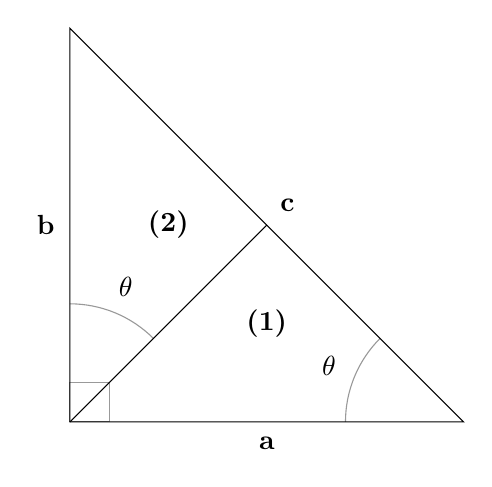
\begin{tikzpicture}[scale=5]
    % Define Edges
    \coordinate (A) at (0,0);
    \coordinate (B) at (1,0);
    \coordinate (C) at (0,1);
    \coordinate (D) at (0.5,0.5);
    % Cycle through
    \draw (A)--(B)--(C)--cycle;
    % Bisection
    \draw (0,0) -- (0.5,0.5);
    % Labels
    \tkzLabelSegment[below=2pt](A,B){\textbf{a}}
    \tkzLabelSegment[left=2pt](A,C){\textbf{b}}
    \tkzLabelSegment[above right=2pt](B,C){\textbf{c}}
    % Label Sections
    \node at (0.5,0.25) {\textbf{(1)}};
    \node at (0.25,0.5) {\textbf{(2)}};
    % Angles
    \tkzMarkRightAngle[fill=none,size=0.1,opacity=.4](C,A,B)
    \tkzMarkAngle[fill=none,size=0.3,opacity=.4](C,B,A)
    \tkzMarkAngle[fill=none,size=0.3,opacity=.4](D,A,C)
    \tkzLabelAngle[pos = 0.37](C,B,A){\(\theta\)}
    \tkzLabelAngle[pos = 0.37](D,A,C){\(\theta\)}
  \end{tikzpicture}
\end{center}

Note by geometric properties, the two smaller triangles (\textbf{(1)} and \textbf{(2)}) are actually similar (infact, all 3 are similar!). Thus, as is shown with $\theta$ being consistent with them both, we can apply our rule of area:

\[
\begin{aligned}
  A_{(0)} & = A_{(1)} + A_{(2)} \\
  c^{2}f(\theta) & = a^{2}f(\theta) + b^{2}f(\theta) \\
  \Aboxed{c^{2} & = a^{2} + b^{2}}
\end{aligned}
\]

\textbf{Question 3}

First, we need to relate the number of rowers with the area of the boat, $A$. This effectively reduces to the square-cubed law; the depth of the boat scales with $n$ so the area must go as $a^{\frac{2}{3}}$. Now, the problem is straight forward if we assume maximum velocity of the boat:
\[
\begin{aligned}
  F & \sim \rho Av^{2} \\
  P & \sim \rho a^{\frac{2}{3}}v^{3} \\
  n & \sim \rho a^{\frac{2}{3}}v^{3} \\
  \Aboxed{v & \sim n^{\frac{1}{9}}\rho^{-\frac{1}{3}}}
\end{aligned}
\]

\textbf{Question 4}

This is simple; we know that distance is inversely proportional to mass in natural units, so we can approximate $r$ as such:
\[ r \sim \frac{1}{m} = \frac{1}{0.938\, \text{GeV}}\cdot 2\times10^{-14}\,\text{Gev}\cdot\text{cm} = 2.132\times10^{-14}\,\text{cm} \]
as required.

\end{document}
